% -- just a two column document
\documentclass[conference]{IEEEtran}

% \usepackage{todonotes}
% \usepackage{cite}
\usepackage{amsmath,amssymb,amsfonts}
\usepackage{algorithmic}
\usepackage{graphicx}
\usepackage{textcomp}
\usepackage{xcolor}
\usepackage{biblatex}
\usepackage{ifthen}
\usepackage{etoolbox}
\usepackage{hyperref}
% \maxdeadcycles=200


% Package for better math typesetting
\usepackage{amsmath}

% Package for custom lists
\usepackage{enumitem}


\addbibresource{ref.bib}

% Package to count todos

% Counter for todos
\newcounter{todocount}
\setcounter{todocount}{0}

% \todo command
\newcommand{\todo}[1]{
  \stepcounter{todocount}
}

% Display todo count
\newcommand{\showtodocount}{%
  \ifthenelse{\value{todocount}=0}{%
    % No todos
    \section*{Todo List}
    No todos.
  }{%
    % Todos found
    \section*{Todo List}
    Total todos: \arabic{todocount}.
  }
}







\title{Hardware Implementation of MNIST digit recognizer using Binary Neural Networks}





\author{
\IEEEauthorblockN{Joshua Azimullah}
\IEEEauthorblockA{5054354\\
j.r.azimullah@tudelft.nl}
\and
\IEEEauthorblockN{Pieter Becking}
\IEEEauthorblockA{4685377\\
PBecking@tudelft.nl}
\and
\IEEEauthorblockN{Christian van den Berg}
\IEEEauthorblockA{00000000\\
email@example.com}
\and
\IEEEauthorblockN{Ioannis Karydis}
\IEEEauthorblockA{5954460\\
ikarydis@tudelft.nl}
}

\begin{document}
\maketitle


\begin{abstract}
\end{abstract}

\todo{general todos}
\todo{work out all todos}
\todo{Each section in the beginning describes what it will say}
\todo{Connecting signal words?}


\section{Introduction}

\subsection{Basic Theory of Binary Neural Networks}


\todo{rewrite this academically -> Binary Neural Networks (BNNs) are an advanced quantization method for neural networks that offers a unique approach to computation. By quantizing weights to 1-bit, BNNs streamline the multiplication process to produce more efficient results. This innovative method allows for hardware efficiency improvements when compared to traditional quantized and floating-point neural networks.}
Binary Neural Networks (BNNs) are the ultimate quantization method for neural networks. There is no way of quantizing a weight to lower than 1-bit. Quantizing to 1-bit opens up a unique new way of computation, since instead of any other number of bits representation, 1-bit multiplication with 1-bit produces only 1 bit. Therefore a multiplication can be modelled as a truth table. This opens the possibility of many hardware efficiency improvements over traditional quantized and floating-point neural nets.


Overall, BNNs offer a promising approach to developing efficient and high-performance neural networks suitable for a wide range of practical applications. BNNs represent a class of neural networks where weights and activations are constrained to binary values, typically \(\{-1, 1\}\). This binarization facilitates significant computational efficiency, particularly in hardware implementations.

% \subsection{Equivalence of Matrix Multiplication and XNOR-Popcount Operations}

In BNNs, matrix multiplication involving binary weights and activations can be effectively implemented using XNOR and popcount operations in hardware. The XNOR operation provides a binary equivalence to multiplication, while the popcount function, which counts the number of ones in the result, corresponds to the summation step in matrix multiplication. This approach is computationally efficient and well-suited to hardware accelerators.

\todo{these refs}
\todo{ref other section}
This equivalence has been detailed in various studies \cite{placeholder1, placeholder2}, highlighting the advantages of BNNs for high-speed and energy-efficient computations in specialized hardware.




\subsection{Contribution \& Scope of the Project}

\todo{Rewrite aim, such that our aim was to first achieve a respectable accuracy of 95\% on the MNIST dataset, and then further improve the design to optimize on area, power and minimum achievable clock speed.}

\todo{rewrite this part also include: we used MNIST dataset (with reference), testset of 10.000 images. -> Our project began with the ambitious goal of achieving a significant milestone: attaining a respectable accuracy rate of 95\% on the renowned MNIST dataset, consisting of handwritten digits [1](cite the page of yann lecun??). This task was conducted using a test set comprising 10,000 images, providing a rigorous evaluation of our model's performance.

Moving forward, our project expanded its scope to encompass the optimization of key design parameters, namely area, power efficiency, and the minimum achievable clock speed. This optimization phase represents a critical contribution, as it delves into the intricate balance between computational efficiency and performance within our system.

By meticulously fine-tuning these aspects, we aim to not only enhance the overall efficiency of our model but also pave the way for future advancements in machine learning hardware. This holistic approach underscores our commitment to not only achieving high accuracy but also ensuring scalability and practicality in real-world applications.

Furthermore, our project covers both the training and inference phases, providing a comprehensive view of the BNN's practical use and performance. This ensures that our analysis extends beyond mere accuracy metrics, offering insights into the model's effectiveness across various operational contexts.}

It covers both training and inference phases, providing a complete view of the BNN's practical use and performance.

\subsection{Outline}
\begin{enumerate}[label=\Roman*.]
    \item INTRODUCTION
    \begin{enumerate}[label=\Alph*.]
        \item \textit{Basic Theory of Binary Neural Networks}
        \item \textit{Contribution \& Scope of the Project}
        \item \textit{Outline}
    \end{enumerate}
    \item OVERVIEW OF BNN ARCHITECTURE
    \begin{enumerate}[label=\Alph*.]
        \item \textit{Training Architecture}
        \item \textit{Inference Network Architecture}
    \end{enumerate}
    \item IMPLEMENTATION OF BNN ARCHITECTURE
        \begin{enumerate}[label=\Alph*.]
            \item \textit{Software implementation}
            \item \textit{Hardware implementation}
            \item \textit{Optimizations}
            \begin{enumerate}[label=\arabic*.]
                \item \textit{Pipelining Popcount}
                \item \textit{LFSR-Based Majority Classifier}
            \end{enumerate}
        \end{enumerate}
    \item RESULTS
        \begin{enumerate}[label=\Alph*.]
            \item \textit{Simulation Setup}
            \item \textit{Demonstration}
            \item \textit{Design metric results}
            \item \textit{General design Trade-Off}
            \item \textit{Hardware Trade-off Results}
            \begin{enumerate}[label=\arabic*.]
                \item \textit{Small section that weight memory is most of the area}
                \item \textit{XNOR popcount}
                \item \textit{Matrix 2}
            \end{enumerate}
            \item \textit{Accuracy Trade-Off}
        \end{enumerate}
    \item CONCLUSIONS
    \begin{description}
        \item APPENDIX
            \begin{enumerate}[label=\Alph*.]
                \item \textit{First matrix multiplication with activation}
                \item \textit{maths second matrix}
            \end{enumerate}
    \end{description}
\end{enumerate}



\todo{written table of contents for coming sections -> DONE}

\section{Overview of BNN Architecture}

\subsection{Training Architecture}
Section \autoref{ref:why_768} provides a rationale for choosing 768 input values over 784, demonstrating superior performance in our specific context.

The architecture of our training network is outlined as follows:
\begin{itemize}
    \item The input vector consists of 768 values, each either -1 or 1.
    \item The first layer performs a matrix multiplication using a weight matrix of size \(1024 \times 768\).
    \item A hardtanh activation function is applied, resulting in output values constrained within the range \(\{-1, 1\}\).
    \item The second layer performs a matrix multiplication with a weight matrix of size \(10 \times 1024\).
    \item The resulting output vector comprises 10 summed values.
    \item The maximum value among these 10 sums is selected as the prediction.
\end{itemize}

\subsection{Inference Network Architecture}
The inference network shares the same mathematical structure as the training network. The primary difference lies in the activation function: the inference network employs a hard activation to constrain outputs strictly to -1 and 1.



\section{Implementation of BNN architecture}
\subsection{Software implementation}
\todo{list learning rate, batch size}

Our BNNs are trained using PyTorch, leveraging the Adam optimizer and CrossEntropy loss function, with one-hot encoded outputs. Prior to training, the input values are rounded to \(\{-1, 1\}\), ensuring the network adapts to these binary inputs. Training is conducted in floating-point representation, with binarization applied post-training.

In the MNIST dataset, the 8-bit input values are pre-processed such that values are mapped to $1$ if $\geq 128$, and to $-1$ otherwise. The HardTanh function is used during training to nudge activations towards hard binary values. 

Parallel evaluations using NumPy, simulating the potential BNN's performance, involve rounding matrices to \(\{-1, 1\}\) to validate that inference based on the matrix multiplications using the rounded values aligns with the outcomes predicted by the PyTorch model.


\subsection{Hardware implementation}

\autoref{fig:overview} shows the hardware architecture of the Binary Neural Network (BNN). 

The XNOR Popcount Evaluator (\autoref{fig:xnor_popcount}) performs the first matrix multiplication and activation by XNORing and popcounting the input vector with the current row of weights. It outputs a bit indicating if the sum is $\geq 384$. The Majority Classifier (\autoref{fig:majority_classifier}) conducts the second matrix multiplication, determining the output by choosing the highest sum among the columns.

In each clock cycle, a row from the first matrix (XNOR Popcount) and a column from the second matrix (Majority Classifier) are processed in parallel. The XNOR Popcount Evaluator is the bottleneck, so the second matrix operation isn't accelerated. 

On reset, both matrix\_1 and matrix\_2 counters reset to 0. These counters, as shown in \autoref{fig:overview}, select the current row and column in the respective matrix register files. The matrix\_1 counter increments each cycle until it completes the register file. 

The XNOR Popcount Evaluator takes the input vector and the current row from weights\_1, XNORs them, and popcounts the result, outputting a bit if the sum $\geq 384$. It also produces a validity bit, initially set low, which counts to a specific count $n$ using an LFSR counter, after which it is set high. This bit is set after $n$ cycles based on the optimization in Section \ref{ref:pipeline_popcount}.

The Majority Classifier activates if the validity bit is set. Upon activation, it increments the matrix\_2 counter after each cycle, resulting in a delay behind the matrix\_1 counter by $n$. No additional enable signal is needed; a reset to 0 starts the prediction process directly. The Majority Classifier also holds a count equivalent to the matrix\_2 count, and when this count equals the hidden size $1024$, the done flag is set high, signaling prediction completion.




\begin{figure}[h]
    \centering
    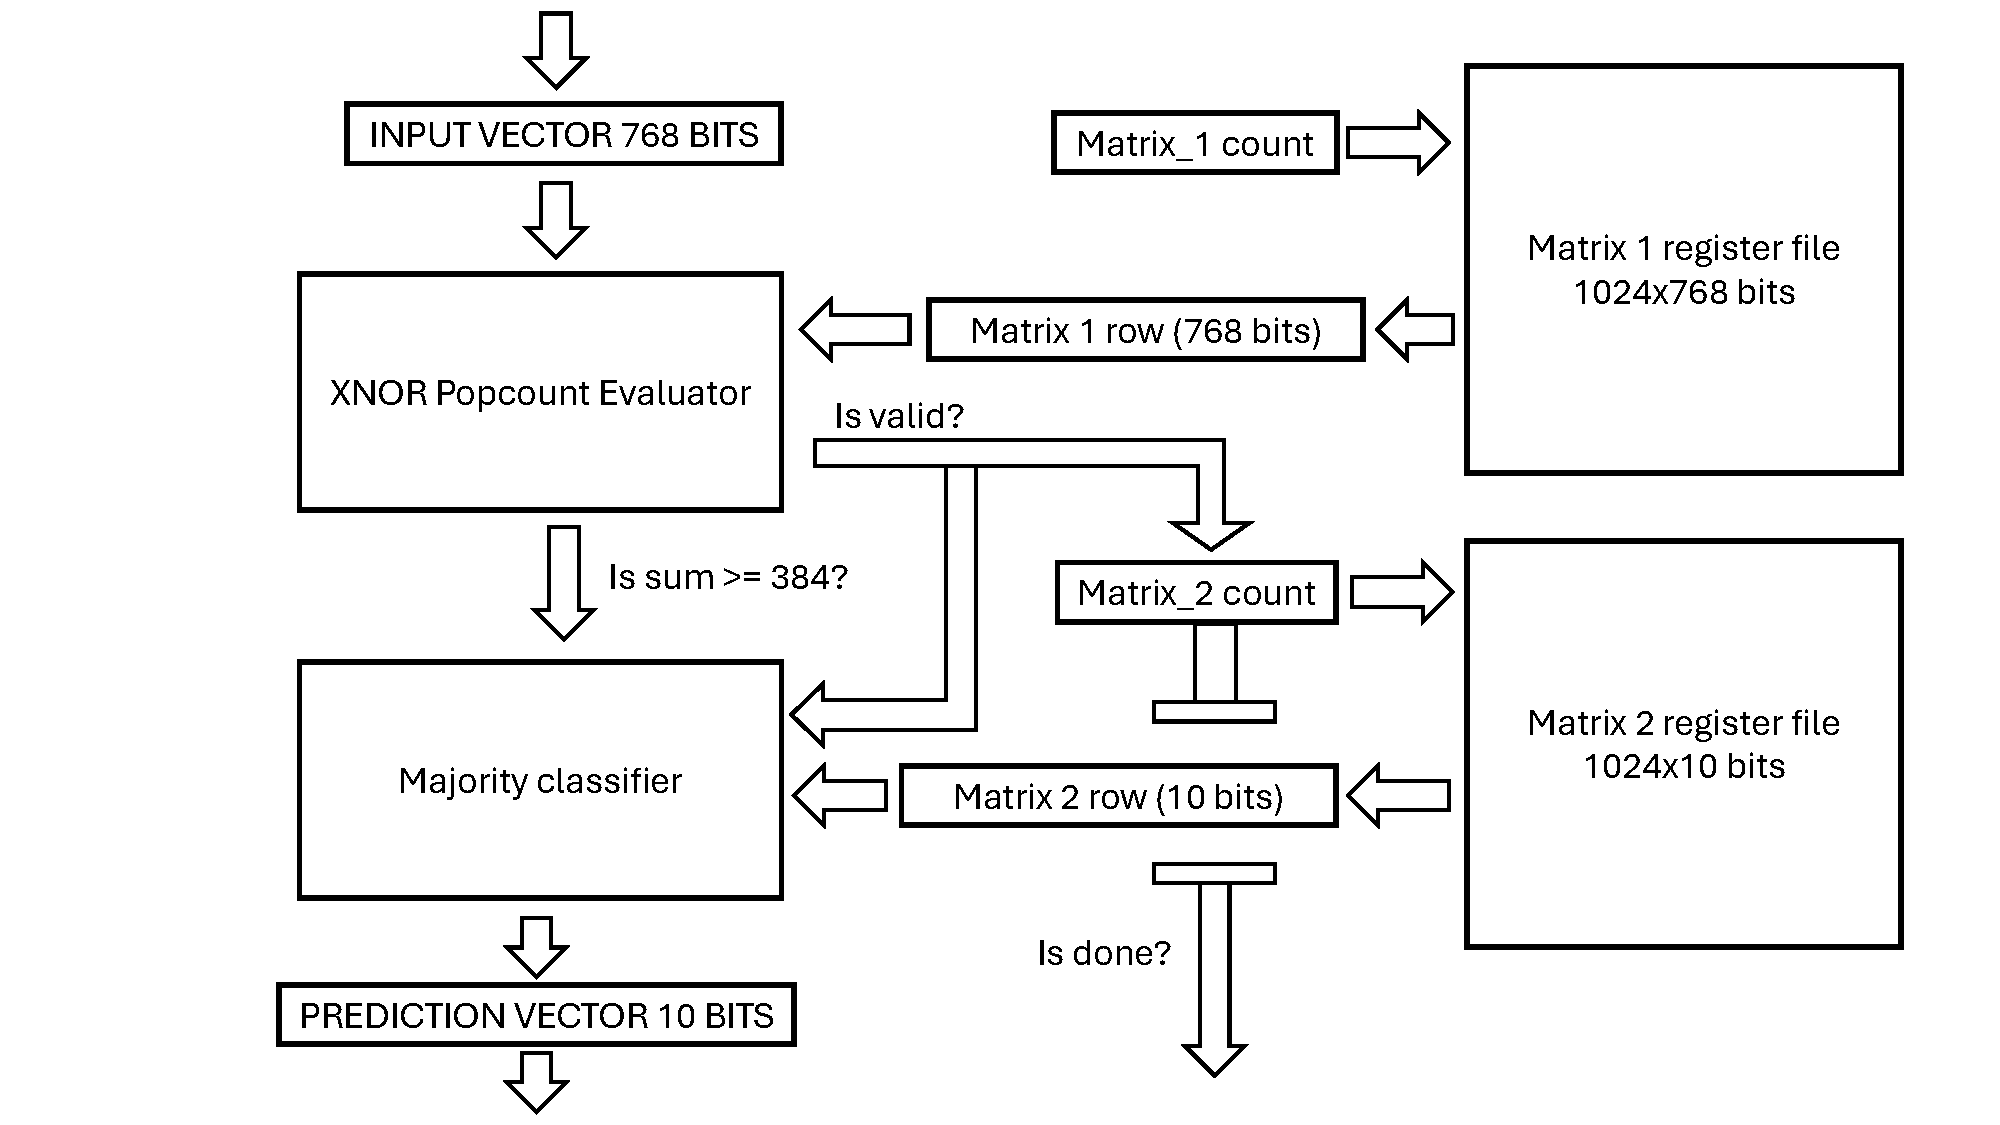
\includegraphics[width=0.4\textwidth]{overview.pdf}
    \caption{Overview of the hardware architecture.}
    \label{fig:overview}
\end{figure}

\begin{figure}[h]
    \centering
    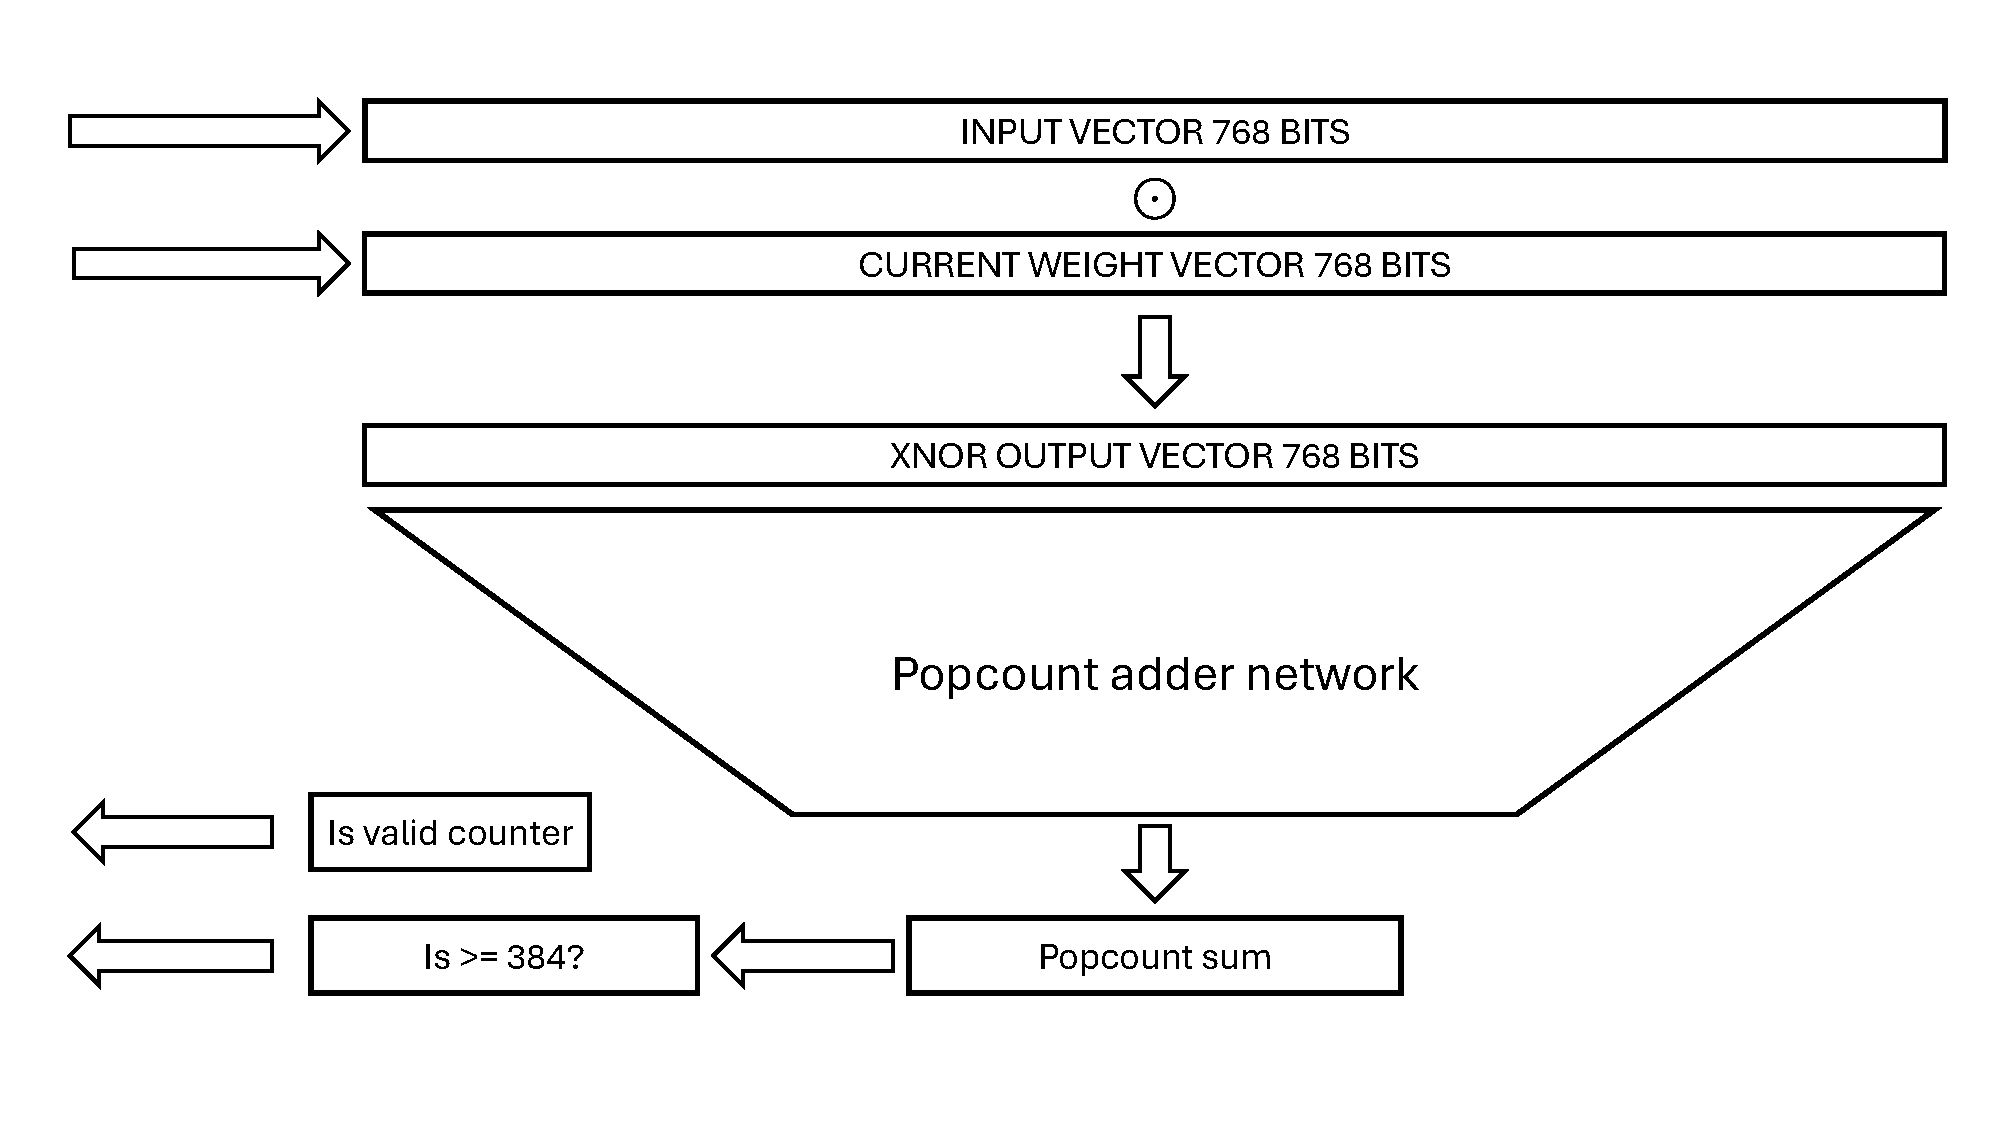
\includegraphics[width=0.4\textwidth]{Xnor_popcount.pdf}
    \caption{XNOR Popcount Evaluator.}
    \label{fig:xnor_popcount}
\end{figure}

\begin{figure}[h]
    \centering
    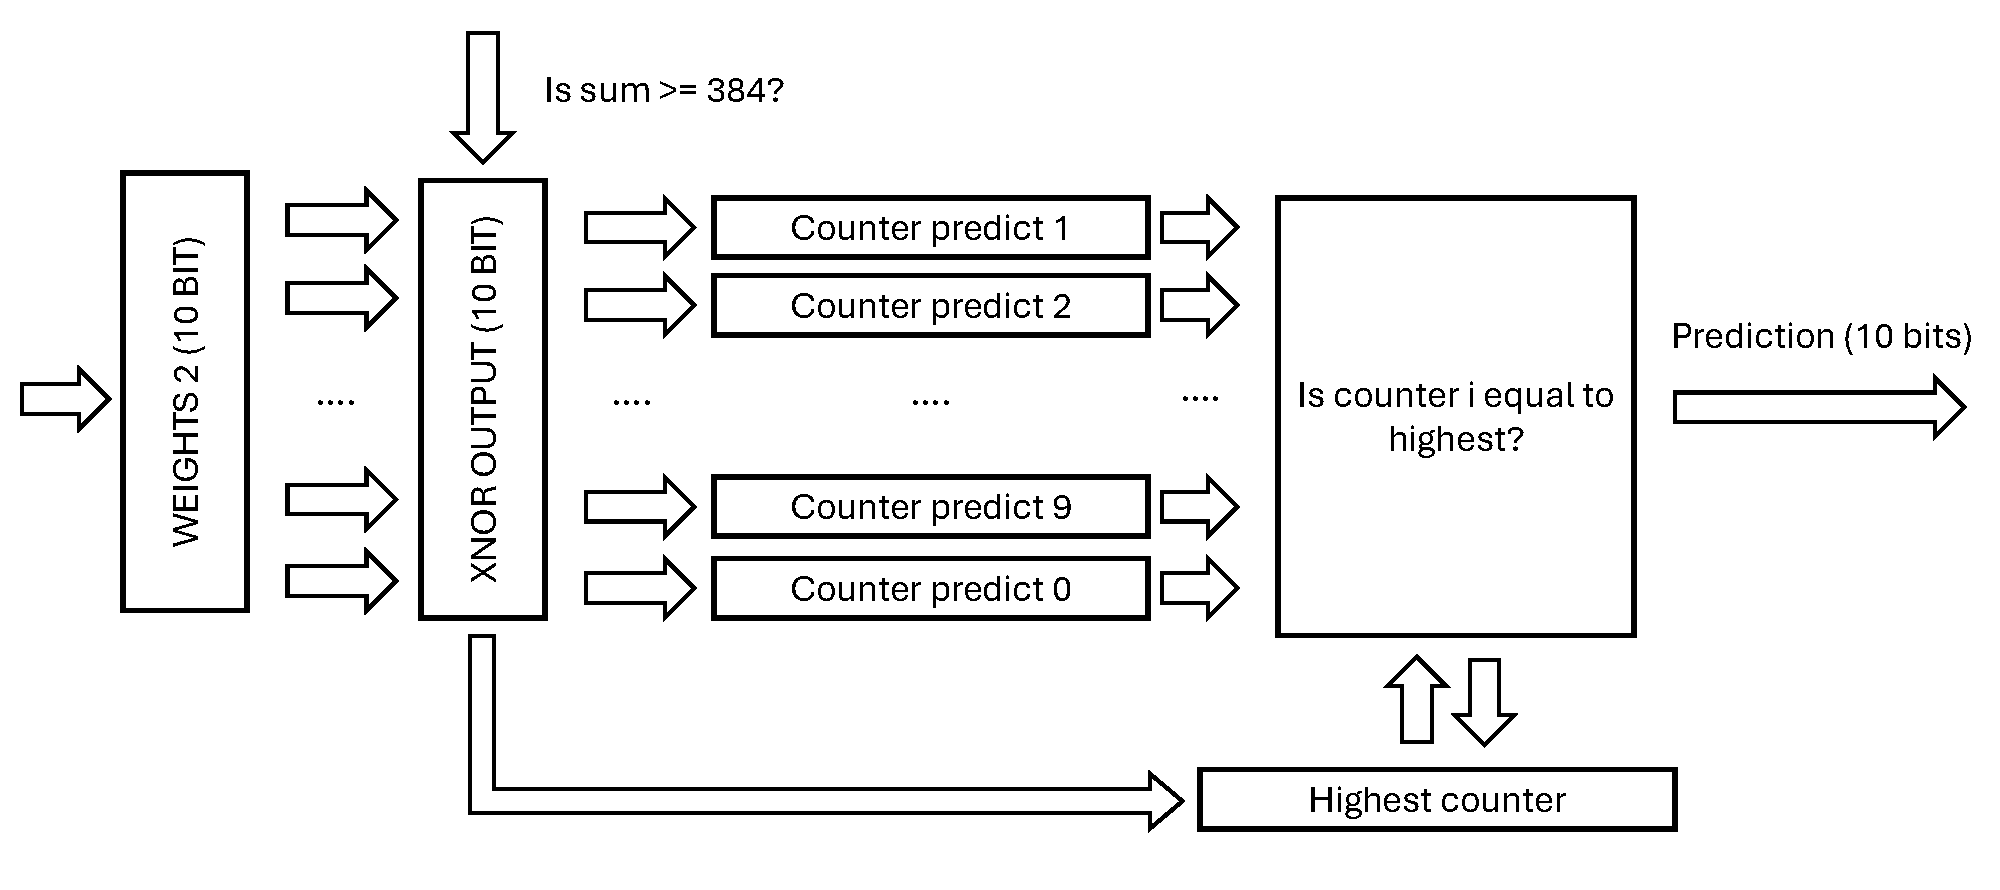
\includegraphics[width=0.4\textwidth]{majority_classifier.pdf}
    \caption{Majority Classifier.}
    \label{fig:majority_classifier}
\end{figure}



\subsection{Optimizations}
\subsubsection{Pipelining Popcount}
\label{ref:pipeline_popcount}

Instead of performing the popcount in a single clock cycle using a large Carry-Save Adder (CSA) network, our exploration in \autoref{ref:exploration_pipelining} determined that a pipelined approach with four registers between the adder stages is optimal. Thus, the popcount result becomes valid after $n=4$ cycles, with subsequent cycles producing new valid sums.

\subsubsection{LFSR-Based Majority Classifier}

Initially, individual counters for each digit were used, along with a tree structure to identify the highest count. However, this structure is redundant if the highest count is tracked dynamically. Each counter is compared against the current highest count. If a counter matches the highest count and is to be incremented, the highest count is updated accordingly. This update is achieved by performing a bitwise AND operation between a 10-bit vector indicating counters equal to the highest count and a 10-bit vector indicating counters to be incremented. An OR reduction of this resultant vector determines if the highest count should increase. 
Ultimately, this approach allows the additional optimization of replacing normal counters with Linear Feedback Shift Register (LFSR) counters, which provide equivalent functionality using less area, as is shown in Section \ref{ref:lfsr_opt}



\section{Results}
\subsection{Simulation Setup}

The initial model, developed in PyTorch, was translated into raw NumPy operations using values of 1 and -1. Upon validation, the NumPy implementation was segmented into the XNOR Popcount and Majority Classifier components.

This segmentation allowed the generation of random test data for both components, output as binary text files containing 0s and 1s. These text files served as inputs for testbenches to validate the functionality of each component individually.

Additionally, text files for input vectors and corresponding labels were generated using the same method. This enabled testing the entire 10,000-image MNIST testset to verify the device's operation.

Simulations were executed using GHDL to accelerate the simulation process and facilitate rapid testing iterations.



\subsection{Demonstration}
\todo{Demonstration show accuracy from simulation}




\subsection{Accuracy Metrics}

\subsubsection{Hidden size Optimization}

since our bnn device uses a sequential method for processing the hidden layer, the hidden size can be precisely adjusted to get the best hidden size for a given accuracy.
Increasing the hidden size both increases the number of clock cycles:  clock cycles inference = hidden size + delay caused by xnor popcount evaluator. where hidden size >> delay cycles>
Furthermore storing the weights as is discussed in Section \ref{ref:overall_minus_rest}, is the largest contributer for area, power and timing. and the hidden size both affects the matrix 1 and 2 linearly in terms of number of bits needed to store.

Therefore any decrease in hidden size causes a big win in terms of performance on all metrics except accuracy.
we first did a overview hidden size exploration to get to the 95\% target first.

At first a global overview was done with the hidden sizes of powers of two: 64,128,256,512,1024,2048,4096
from here it was found that from 1024 it was sufficient since an accuracy of 95\% was achieved seen in \autoref{fig:line_graph_global}

next for optimization sake every interval of 32 was tested in between, \autoref{fig:bar_max_achieved_accuracy} shows the max achieved accurcacy for each.




% \todo{why not CNN decision: would probably require somewhere a linear layer anyways, or a large number of layers vastly reducing speed}
% \todo{somewhere needs to be put a better reasoning why 2 matrices are more efficient: either have 1024 counters = excessive or 1024x768 counts which is slow and area gains are low}
% The initial goal of our Binary Neural Network (BNN) architecture was to achieve a high level of performance using a single matrix for computations. However, this approach did not meet the target accuracy of 95\%, necessitating exploration of alternative designs.
% Subsequent experiments with two matrices in the network structure suggested that this configuration could offer a similar level of computational efficiency while potentially improving accuracy. 
% \textit{Results pending. This section will present accuracy metrics for different network configurations once available.}
% \todo{lower hidden size, would drop accuracy too much}
% \todo{lower input size also}
 






 

% \todo{subsection accuracy}

% Due to our rigorous testbenches, the accuracy from the raw numpy matrices and the testbench simulation was exactly equal.


\subsection{Hardware metric results}

- text showing overall area, power, timing

\todo{Overall}
  \todo{subsection area}
  \todo{subsection power}
  \todo{subsection timing}

\label{ref:overall_minus_rest}
\todo{Overall - rest} % register files part + counters
  \todo{subsection area}
  \todo{subsection power}
  \todo{subsection timing}

\todo{Theoritical inference performance}

\subsection{Hardware Trade-off Results}

	% - [ ] full design
	% 	- [ ] note on how memory is most of the area
\subsubsection{XNOR popcount}
\label{ref:why_768}
% To further optimize the input dimensions, we reduced the number of inputs from 784 to 768 by dropping the last 16 inputs. This simplification leverages the powers of two, specifically \(768 = 512 + 256 = 2^9 + 2^8\), which can simplify the hardware and align more efficiently with binary operations. This reduction did not impact performance.

\todo{XNOR Popcount Evaluator}
  \todo{subsection area}
  \todo{subsection power}
  \todo{subsection timing}
\label{ref:exploration_pipelining}
\todo{Explanation of results:}
\todo{0 levels and 1 levels a wide number of valid divisors of 768 were tested and shown her}
\todo{2 and 3 levels have too large exploration space thus first a reasonable setup was chosen and then for each additional test, only the part where the lowest slack was changed}

\todo{final choice for design}

	% - [ ] xnor popcount exploration
	% 	- [ ] direct csa tree
	% 	- [ ] 1 level
	% 	- [ ] 2 levels
	% 	- [ ] 3 levels

\subsubsection{Majority classifier}
\label{ref:lfsr_opt}

\todo{Majority Classifier non lfsr}
  \todo{subsection area}
  \todo{subsection power}
  \todo{subsection timing}
\todo{Majority Classifier with lfsr optimization}
  \todo{subsection area}
  \todo{subsection power}
  \todo{subsection timing}






\section{Discussion}
	%   - [ ] accuracy differences were not that great and partially due to random chance
	% - [ ] Hyperparameter tuning might be overfitting on the testset

	% - [ ] Rationale
	%   - [ ] somewhere needs to be put a better reasoning why 2 matrices are more efficient: either have 1024 counters = excessive or 1024x768 counts which is slow and area gains are low
	% 	- [ ] why not CNN decision: would probably require somewhere a linear layer anyways, or a large number of layers vastly reducing speed
	% 	- [ ] Small section that weight memory is most of the area
	%     - [ ] section on hardware possible strategies given Fully connected bnn
	% 	    - [ ] subsubsection strategy do everything sequentially
	% 	    - [ ] subsubsection strategy do everything in parallel in one tick
	% 	    - [ ] subsubsection strategy mixed approach, since parallel would be huge and sequentially would be unneccesary slow for little area and power gains due to weights storage that is mandatory

\section{Conclusions}
	- [ ] exploration of multiple hidden sizes was very benificial
	- [ ] timing bottleneck mostly from memory

\todo{future work}
	- [ ] subsection better memory library
	- [ ] subsection also try 729 as input size for xnor popcount csa network
	- [ ] subsection double is done



\appendix

\section{Mathematical Foundations for Hardware Implementations}

\label{appendix:bnn_maths}

\subsection{First matrix multiplication with activation}

This section demonstrates that performing matrix-vector multiplication followed by a hard activation is equivalent to using XNOR operations, popcount, and a subsequent comparison.
The matrix-vector multiplication \(\mathbf{A} \mathbf{b}\) shown in Equation \ref{eq:matrix_vector_multiplication} results in a vector \(\mathbf{c}\). Each element \(c_i\) of this vector is obtained by the dot product of the \(i\)-th row of matrix \(\mathbf{A}\) with vector \(\mathbf{b}\), as described in Equation \ref{eq:dot_product}. This can be further expanded into component-wise multiplication and summation (Equation \ref{eq:component_wise_dot}). When elements \(a_{ij}\) and \(b_j\) are binary (\(1\) or \(-1\)), we map them to \(1\) and \(0\) respectively, as shown in Equation \ref{eq:mapping}, enabling the use of XNOR for the multiplication, as described in Equation \ref{eq:xnor}.

\begin{figure}[h]
    \centering
    \begin{equation}
    \mathbf{c} = \mathbf{A} \mathbf{b}
    \label{eq:matrix_vector_multiplication}
    \end{equation}

    \begin{equation}
    c_i = \sum_{j=1}^n a_{ij} b_j
    \label{eq:dot_product}
    \end{equation}

    \begin{equation}
    c_i = \sum_{j=1}^n (a_{ij} \cdot b_j)
    \label{eq:component_wise_dot}
    \end{equation}

    \begin{equation}
    a'_{ij} = \begin{cases}
    1 & \text{if } a_{ij} = 1 \\
    0 & \text{if } a_{ij} = -1
    \end{cases}, \quad
    b'_j = \begin{cases}
    1 & \text{if } b_j = 1 \\
    0 & \text{if } b_j = -1
    \end{cases}
    \label{eq:mapping}
    \end{equation}

    \begin{equation}
    a_{ij} \cdot b_j = \text{XNOR}(a'_{ij}, b'_j)
    \label{eq:xnor}
    \end{equation}

    \caption{Matrix-vector multiplication and equivalent dot product representation.}
    \label{fig:matrix_vector_multiplication}
\end{figure}


\begin{figure}[h]
    \centering
    \begin{equation}
    c = \sum_{i=1}^n a_i b_i
    \label{eq:dot_product_sum}
    \end{equation}

    \begin{equation}
    c = \left|\{c_i \mid c_i = 1\}\right| - \left|\{c_i \mid c_i = -1\}\right|
    \label{eq:dot_product_count}
    \end{equation}

    \begin{equation}
    |\{c_i \mid c_i = -1\}| = n - |\{c_i \mid c_i = 1\}|
    \label{eq:negative_count}
    \end{equation}

    \begin{equation}
    a \cdot b = 2 \left|\{c_i \mid c_i = 1\}\right| - n
    \label{eq:dot_product_simplified}
    \end{equation}

    \begin{equation}
    \text{activation}(c) = \begin{cases}
    1 & \text{if } 2 \left|\{c_i \mid c_i = 1\}\right| \geq n \\
    -1 & \text{otherwise}
    \end{cases}
    \label{eq:activation_function}
    \end{equation}

    \begin{equation}
    \text{activation}(c) = \begin{cases}
    1 & \text{if } \left|\{c_i \mid c_i = 1\}\right| \geq \frac{n}{2} \\
    -1 & \text{otherwise}
    \end{cases}
    \label{eq:activation_function_half}
    \end{equation}

    \begin{equation}
    \text{activation}(a \text{ XNOR } b) = \begin{cases}
    1 & \text{if } \text{popcount}(a \text{ XNOR } b) \geq \frac{n}{2} \\
    -1 & \text{otherwise}
    \end{cases}
    \label{eq:activation_xnor}
    \end{equation}

    \caption{Dot product calculation and activation function.}
    \label{fig:dot_product_activation}
\end{figure}

In Figure \ref{fig:dot_product_activation}, Equation \ref{eq:dot_product_sum} sums the products of the components. Equation \ref{eq:dot_product_count} translates the sum into a count of \(1\)s and \(-1\)s. The total count of \(-1\)s can be expressed as the complement of the count of \(1\)s (Equation \ref{eq:negative_count}). The dot product simplifies to Equation \ref{eq:dot_product_simplified}. The activation function (Equation \ref{eq:activation_function}) sets the output based on the threshold condition, which can also be expressed equivalently as shown in Equation \ref{eq:activation_function_half}. This is related to the XNOR operation in Equation \ref{eq:activation_xnor}, where the activation depends on the population count of the XNOR operation being greater than or equal to half the length of the vector.


\subsection{maths second matrix}
\todo{subsubsection maths is same but now the actual highest popcount needs to be found}





\printbibliography

\showtodocount

\newpage

\end{document}






